%UNLIKE IN A REGULAR TEX FILE, DON'T PUT ANY PREAMBLE MATERIAL HERE
\section*{Abstract}
We present preliminary studies into the development of efficient and effective strategies for the usage of LSST in optical follow-up of gravitational wave events. Specifically, we focus on the detection and characterization of kilonovae across a wide range of ejecta properties and composition. We show that the main LSST survey will achieve an average efficiency for kilonova detection of \apx3\%, with only a handful of sources characterized well enough for detailed study. In contrast, triggered target-of-opportunity follow up with a time investment of just 1 hour per event will be able to detect and characterize the brightest kilonova models, provided observations commence promptly after the GW trigger. This suggests that LSST has the opportunity to play an important role in the growth of multi-messenger astronomy by facilitating highly efficient kilonova searches.

\clearpage
\section{Introduction}
\label{sec:ch6_intro}
The discovery of an optical counterpart associated with the the binary neutron star merger GW170817 was a watershed moment in the development of joint gravitational wave and electromagnetic (GW-EM) astronomy \citep{LIGOGW170817,LIGOMMAPaper,Arcavi+17,Coulter+17,GW170817DECam,Valenti+17}. Subsequent modeling of the optical light curves revealed behavior consistent with that of a kilonova \citep{Cowp+17,Kilpatrick+17,Tanaka+17,Villar+17b, Tanaka+18}, an optical/NIR transient expected to accompany compact object mergers involving at least one neutron star \citep[see e.g.,][]{Metzger2017}. The discovery of this optical transient has opened up numerous new and exciting science possibilities. These include studies into the host galaxy \citep[NGC4993, see e.g.,][]{Blanchard+17,Cantiello+18}, constraining the neutron star equation of state \citep[see e.g.,][]{Radice+18}, and even making independent measurements of the local Hubble Constant \citep[H$_0$, see e.g.,][]{LIGOH0,Guidorzi+17}.

If we wish to build upon the success of GW170817 and push into new realms of joint GW-EM science then we must work to facilitate future detections of both gravitational wave sources {\em and} their associated electromagnetic counterparts. A key component of future searches for gravitational wave events is improving the ability of the interferometer network to localize sources on the sky. Over the next several years, as both Advanced LIGO and Virgo reach their design sensitivity, it is expected that they will be able to localize compact binary mergers to sky areas of approximately tens to hundreds of deg$^2$ \citep{LIGOLocalization,ChenHolz16}. Major improvements to sky localization will continue over the next decade as two additional interferometers, KAGRA in Japan \citep{KAGRA} and LIGO-India \citep{LIGOIndia}, join the network. In this five detector regime, compact binary mergers will be localized to just $\apx10$~deg$^2$ \citep{Fairhurst2014,ChenHolz16}.

Similarly, improving our ability to identify electromagnetic counterparts in these localizations will rely on using the next generation of optical facilities that are soon to be coming online. One such facility, the Large Synoptic Survey Telescope \citep[LSST,][]{Ivezic+09}, will be the premiere time-domain instrument in the Southern hemisphere during the next decade. LSST boasts an 8.4-m primary mirror and a 9.6 deg$^2$ field-of-view. This powerful combination of large aperture and wide field-of-view makes LSST uniquely suited to the task of gravitational wave follow-up. The field-of-view is particularly well matched to the expected localization regions allowing LSST to observe a high fraction of the localization probability in just one or two pointings.

Of particular importance is the development of efficient and effective strategies for gravitational wave follow-up with LSST. This first involves understanding both the rate and properties of kilonovae detected in the LSST main survey. This was investigated by \citet{Scolnic+18} who injected model light curves of the kilonova associated with GW170817 \citep[hereafer just ``GW170817" for simplicity][]{Cowp+17} into the LSST cadence. They found that LSST should detect $\apx7$ GW170817-like kilonovae per year during the ten year main survey. However, these kilonovae were observed only a few times per event, leading to poorly-sampled light curves. As a result, real-time identification and modeling of these kilonovae will be difficult. Furthermore, these kilonovae are detected far beyond the sensitivity horizon for LIGO, meaning that an association between these kilonovae and a gravitational wave detection is unlikely. This suggests that triggered target-of-opportunities may be a more promising approach.

Here we expand on the groundwork established by \citet{Scolnic+18} along two new avenues. First, we expand the range of kilonovae models considered in the LSST main survey. This is accomplished by considering a wider range of ejecta masses and composition to fully explore the potential range of kilonovae brightness and timescales. Second, we expand beyond the main survey cadence to discuss the benefits of targeted target-of-opportunity (ToO) observations when compared to the main survey.

%and explore the detectability of kilonovae in triggered target-of-opportunity follow-up observations. We explore not only the ability of such observations to detect kilonovae, but also identify and characterize their behavior. 

This work is organized as follows: In \cref{sec:ch6_models} we describe the expanded range of kilonovae models used in our simulated observations. In \cref{sec:ch6_obs} we describe our methodology for simulating LSST observations using both OpSim for the main survey cadence and SNANA for target-of-opportunity observations. In \cref{sec:ch6_analysis} we present the results of our simulated observations. Lastly, discussions and conclusions are presented in \cref{sec:ch6_conc}.

All magnitudes presented in this work are given in the AB system unless otherwise noted. Cosmological calculations are performed using the cosmological parameters $H_0 = 67.7$ km s$^{-1}$ Mpc$^{-1}$, $\Omega_M = 0.307$, and $\Omega_{\Lambda} = 0.691$ \citep{Planck2016}.

\clearpage
\section{Kilonova Models}
\label{sec:ch6_models}
A kilonova is an isotropic optical/NIR thermal transient produced by the merger of a compact object binary containing at least one neutron star such as a binary neutron star (BNS) or neutron star-black hole binary (NS-BH). In either scenario, the merger produces a small amount of ejecta ($\Mej \lesssim 0.1 \msun$), which is typically neutron-rich. As the ejecta expands from nuclear densities, it will synthesize heavy elements via $r$-process nucleosynthesis. These heavy nuclei are unstable and will decay back to stability depositing energy into the ejecta which powers the kilonova emission \citep{LP98,Metzger+10,BarnesKasen13,TanakaHotokezaka13,Metzger2017}.

The exact nature of this kilonova emission depends strongly on the composition of the ejecta, specifically the neutron-richness which is parametrized by the electron fraction ($Y_e$). If the material is very neutron-rich ($Y_e \lesssim 0.3$), then the ejecta will undergo strong $r$-process nucleosynthesis, producing very heavy elements ($A > 140$), particularly those in the lanthanide and actinide series. As a result of these heavy elements, the ejecta will have a high opacity $(\kappa \gtrsim 10 \cspg)$. The resulting ``red" kilonova will then be faint with a peak bolometric luminosity of $L_p \apx10^{40}-10^{41} \ergs$, red ($i-z \gtrsim 0$), and exhibit a timescale of $t_p \apx1$ week \citep{BarnesKasen13,TanakaHotokezaka13}. If instead the material is less neutron-rich ($Y_e \gtrsim 0.3$), then the ejecta will undergo light $r$-process nucleosynthesis, producing Fe-group and light $r$-process elements ($A \lesssim 140$), and the ejecta will have a lower opacity $(\kappa \apx0.1 \cspg)$. The resulting ``blue" kilonova will be brighter $L_p \apx10^{41}-10^{42} \ergs$, bluer ($i-z \lesssim 0$), and exhibit a shorter timescale of $t_p \apx1$ day \citep{Metzger+10,MetzgerFernandez14}.

In practice, the observed kilonova will exhibit some combination of both ``red" and ``blue" features. This behavior was seen in the kilonova associated with GW170817, where the multi-band optical/NIR light curve was best described by a three-component model consisting of ``red"  $(\kappa \apx10 \cspg)$, ``purple"  $(\kappa \apx3 \cspg)$, and "blue"  $(\kappa \apx0.1 \cspg)$ $r$-process powered components. This three-component approach was first suggested by \citet{Tanaka+17} as a good approximation to the more complex opacity behavior seen in detailed radiative transport simulations. The three-component approach is also physically motivated as the different emission components may arise from different sources of ejecta present in the merger. The ``blue`` emission may arise from neutron-poor ejecta in the polar region where material is shock-heated during the NS collision \citep{Oechslin+07,Bauswein+13a,Sekiguchi+16} or if the ejecta is irradiated by neutrinos from a long-lived merger remnant \citep{FernandezMetzger13,Just+15,Kasen+15}. The ``purple" and ``red" emission may arise from ejecta produced in the tidal tails during merger \cite{Rosswog+99,Hotokezaka+13} or wind outflows from a post-merger accretion disk \citep{Just+15,SiegelMetzger17}. However, it is currently unknown if the behavior observed in the multi-band light curves of GW170817 will be seen for all kilonovae. For example, if the ``blue" emission is indeed constrained to the polar regions of the ejecta then it will not be observable at all viewing angles, whereas the more isotropic ``red" emission from tidal tails or post-merger disks will be ubiquitous in observations.

We explore this potential diversity in kilonovae emission by producing a grid of models that cover a range of ejecta parameters. We generate synthetic spectral energy densities (SEDs) for kilonovae spanning $2-15$ \micron\ using the {\tt rprocess} model built-in to the \mosfit\ light curve fitting package \citep{Guillochon+17b,Nicholl+17b}. The {\tt rprocess} model is discussed in \citet{Villar+17a} and describes a single-component kilonovae \citep{Metzger2017} parametrized by the ejecta mass ($\Mej$), velocity ($\vej$), and opacity ($\kappa$). We produce models at the extremes of the mass grid outlined in Table 1 of \citet{Barnes+16} with $\Mej = [0.001, 0.05]\,\msun$. For each choice of ejecta mass, we produce both ``red" $(\kappa \apx10 \cspg)$ and ``blue" $(\kappa \apx0.1 \cspg)$ models. Lastly, we fix $\vej$ at 0.3c for the ``blue" kilonova and 0.1c for the ``red" kilonova. We combine permutations of these SEDs to produce a final set of four models that cover a wide dynamic range in both brightness and color. These models are presented in \cref{tab:ch6_models}.

\begin{deluxetable}{cccccccc}
\singlespace
\tabletypesize{\footnotesize}
\tablecolumns{12}
\tablewidth{0pt}
\tablecaption{Model Kilonova SED Parameters
	          \label{tab:ch6_models}}
\tablehead{
\colhead{Model} &
\colhead{Name} &
\colhead{$\Mej^{\rm blue}$} &
\colhead{$\vej^{\rm blue}$} &
\colhead{$\kappa^{\rm blue}$} &
\colhead{$\Mej^{\rm red}$} &
\colhead{$\vej^{\rm red}$} &
\colhead{$\kappa^{\rm red}$} \\
\colhead{} &
\colhead{} &
\colhead{($\msun$)} &
\colhead{(c)} &
\colhead{($\cspg$)} &
\colhead{($\msun$)} &
\colhead{(c)} &
\colhead{($\cspg$)} 
}
\startdata
1 & {\tt h\_blue\_h\_red} & 0.05 & 0.3 & 0.1 & 0.05 & 0.1 & 10 \\
2 & {\tt h\_blue\_l\_red} & 0.05 & 0.3 & 0.1& 0.001 & 0.1 & 10 \\
3 & {\tt l\_blue\_h\_red} & 0.001 & 0.3 & 0.1& 0.05 & 0.1 & 10 \\
4 & {\tt l\_blue\_l\_red} & 0.001 & 0.3 & 0.1& 0.001 & 0.1 & 10 \\
\enddata
\tablecomments{Model parameters for the four synthetic kilonovae SEDs produced using the {\tt rprocess} model in \mosfit\ \citep{Guillochon+17b,Nicholl+17b,Villar+17a}. The individual SED components are produced as described in \cref{sec:ch6_models} and then coadded in luminosity space to produce the final ``red+blue" kilonovae.}
\end{deluxetable}

The four kilonova models described above represent the possible extremes of kilonovae behavior. Constructing models for intermediate cases is more difficult. The exact nature of the combined ``red" and ``blue" components depends strongly on assumptions such as the geometry and velocity structure of the ejecta or possible mixing between ejecta components. We instead use GW170817 as an empirical representation of a kilonova observed with blended ``red" and ``blue" features. We generate model SEDs for GW170817, over the same wavelength range as our fiducial models with \mosfit, using the best-fit parameters from the three-component model of \citep{Villar+17b}. These five models will form the basis of sources injected into our simulated observations.

\clearpage
\section{Simulated Observations}
\label{sec:ch6_obs}

%In this work, we consider the detectability and characterization of kilonovae in two unique observing situations. The first is the serendipitous detection of kilonovae in the LSST main survey independent of a GW trigger from LIGO. The second is triggered target-of-opportunity observations conducted by LSST in response to a GW trigger. We generate simulated observations for both scenarios as follows: 
%
%\subsection{Main Cadence Simulations With OpSim}
%\label{sec:ch6_opsim}

We produce simulated observations of kilonovae in the LSST main cadence using the LSST Operations Simulator \citep[OpSim,][]{OpSim1,OpSim2}. This is a publicly available package designed to produce realistic simulations of LSST scheduling and imaging over the ten year duration of the survey. These simulations provide realistic information about observations including cadence and science program requirements, observing conditions due to telescope or environmental factors, and image characteristics. We use the most recent OpSim reference run ({\tt minion\_1016}) to produce a catalog of observations including times, sky position, photometric errors, and limiting magnitudes.

We inject our kilonova model into this database of observations. For each injection, we uniformly choose a random model from the five described in \cref{sec:ch6_models}. The chosen model is injected at a randomly selected sky position and time, chosen uniformly. The model is injected at a random  
distance over a volume defined by the maximal LIGO BNS detection radius $(\apx450$ Mpc) in distance bins of 50~Mpc. Since it is not guaranteed that LSST with be looking at the chosen position and time where the source is injected, we continually inject sources until we have 100 kilonovae in each distance bin. This method allows more robust statistics at smaller distances compared to a volume-weighted injection scheme and allows us to compute LSST all-sky efficiencies and determine the total number of expected transients detected during the survey (see \cref{sec:ch6_opsim_results}).

%\subsection{Target of Opportunity Simulations With SNANA}
%\label{sec:ch6_snana}
%We parametrize our triggered target-of-opportunity (ToO) strategies based on the expected time investment per night and total number of nights spent observing. In this work we assume that the typical LIGO localization region is \apx10~deg$^2$ and can therefore be observed in just two LSST pointings, which are necessary to cover chip gaps in the CCD mosaic. We assume that each pointing consists of $grizY$ observations lasting 30~s each with per filter overheads of 90~s. This puts the total time investment at 10 minutes per pointing, or 20 minutes per night. We assume 7 nights of observing for a total telescope time investment of \apx2.5~hours. To test the effect of rapid cadence observations, we include a second epoch on the first night, taken 3 hours after the initial epoch.
%
%We simulate these ToO observations using the SNANA public software package \citep{SNANA}. SNANA is a supernova analysis and simulation package designed to produce realistic supernovae light curves for the optimization of time-domain surveys and extraction of cosmological parameters. SNANA generates these light curves using a model transient SED, realistic filter transmission functions, and a database of observation dates and conditions. We run SNANA using our kilonova model SEDs and LSST filter transmission functions, and generate the database of observing conditions by pulling key information from the OpSim simulations (e.g., sky noise, PSF, observed zero point, see \cref{sec:ch6_opsim}). We then mutate the observing dates to match those required for our ToO cadence described above.
%
%We inject kilonova following the same procedure outlined in \cref{sec:ch6_opsim} with several key differences. First, we do not inject sources at randon sky locations, but instead at the location LSST is observing in the SNANA database. Second, in order to probe a realistic range of response times for the ToO trigger, we inject kilonova at a uniformly sampled time from 3--24 hours prior to the first epoch. Lastly, SNANA randomly selects an injection distance using a volume-weighted scheme to generate a realistic distribution. We therefore, inject 10,000 kilonovae across the entire volume ($D_L \apx450$~Mpc) to ensure that we have enough nearby sources. Since the distance injection in SNANA is based on redshift, a handful of sources end up with a distance greater than 450~Mpc. To maintain consistency with our OpSim volume, we truncate these sources leaving a final sample of 9171 light curves for our analysis in \cref{sec:ch6_snana_results}.

\section{Analysis}
\label{sec:ch6_analysis}
The analysis of the simulated light curves presented here is focused along two major lines of thought. In the context of kilonovae detected in the LSST main survey, we are primarily concerned with not only how many kilonovae will be detected, but also how many of those detections will yield enough light curve information to make statements about the ejecta (e.g., mass, velocity, composition). We then wish to compare these results to qualitative expectations for a targeted ToO program.

%In the context of targeted ToO observations, we are not only concerned with these issues of detection and characterization, but also the impact of program design (e.g., telescope time investment) on the science returns.

\subsection{Results from OpSim}
\label{sec:ch6_opsim_results}
We first define our criteria for the detection of a kilonova along with the key information required for better characterization of the kilonova behavior:
\begin{enumerate}
\item We define a ``detection" as any light curve with at least 3 observations that achieve a S/N $> 5$. These observations can be across any combination of times and filters.
\item We define a ``rise" as any light curve that exhibits brightening between two observations. This light curve must also satisfy the requirements for a detection. Due to the potentially longer cadence of these observations, the brightening does not need to be observed in the same filter.
\item We define a ``color" measurement as any light curve with S/N $> 5$ in two independent filters. As with the rise criterion, this light curve must also satisfy the requirements for a detection.
\end{enumerate}

Applying these criteria across all distances and all models we find that out of 3653 injected kilonova we detect 123 kilonovae giving a total efficiency of $3\%$. If we exclude the 2553 kilonovae that were injected at times and sky locations not observed by LSST then this efficiency increases to $11\%$. Furthermore, of the 123 kilonovae detected in our survey we able to obtain information about the rise for 62 events and color information for 99 events. Lastly, we are able to obtain both color and rise information for 52 events. These numbers are shown as a function of distance in \Cref{fig:ch6_eff_hist} and as a function of kilonova model in \cref{tab:ch6_eff}.

\begin{deluxetable}{ccccccc}
\singlespace
\tabletypesize{\footnotesize}
\tablecolumns{12}
\tablewidth{0pt}
\tablecaption{LSST Main Survey Efficiencies
	          \label{tab:ch6_eff}}
\tablehead{
\colhead{Model} &
\colhead{Name} &
\colhead{$N$} &
\colhead{$N_{\rm det}$} &
\colhead{$N_{\rm rise}$} &
\colhead{$N_{\rm color}$} &
\colhead{$N_{\rm both}$}
}
\startdata
1 &  GW170817 & 172 & 29 & 16 & 24 & 13 \\
2 & {\tt h\_blue\_h\_red} & 167 & 47 & 21 & 37 & 18 \\ 
3 & {\tt h\_blue\_l\_red} & 165 & 24 & 14 & 16 & 10 \\
4 & {\tt l\_blue\_h\_red} & 212 & 0 & 0 & 0 & 0 \\
5 & {\tt l\_blue\_l\_red} & 181 & 0 & 0 & 0 & 0
\enddata
\tablecomments{Detection efficiencies for each kilonova model. $N$ denotes the total number of models injected. $N_{\rm det}$ denotes the total number of kilonovae detected. $N_{\rm rise}$ denotes the total number of kilonovae for which brightening was detected. $N_{\rm color}$ denotes the total number of kilonovae for which color information was obtained. Lastly, $N_{\rm both}$ denotes the total number of sources for which both brightening and color information is available.}
\end{deluxetable}

%\begin{figure}[!t]
%\begin{center}
%\hspace*{-0.1in}
%\scalebox{1.}
%{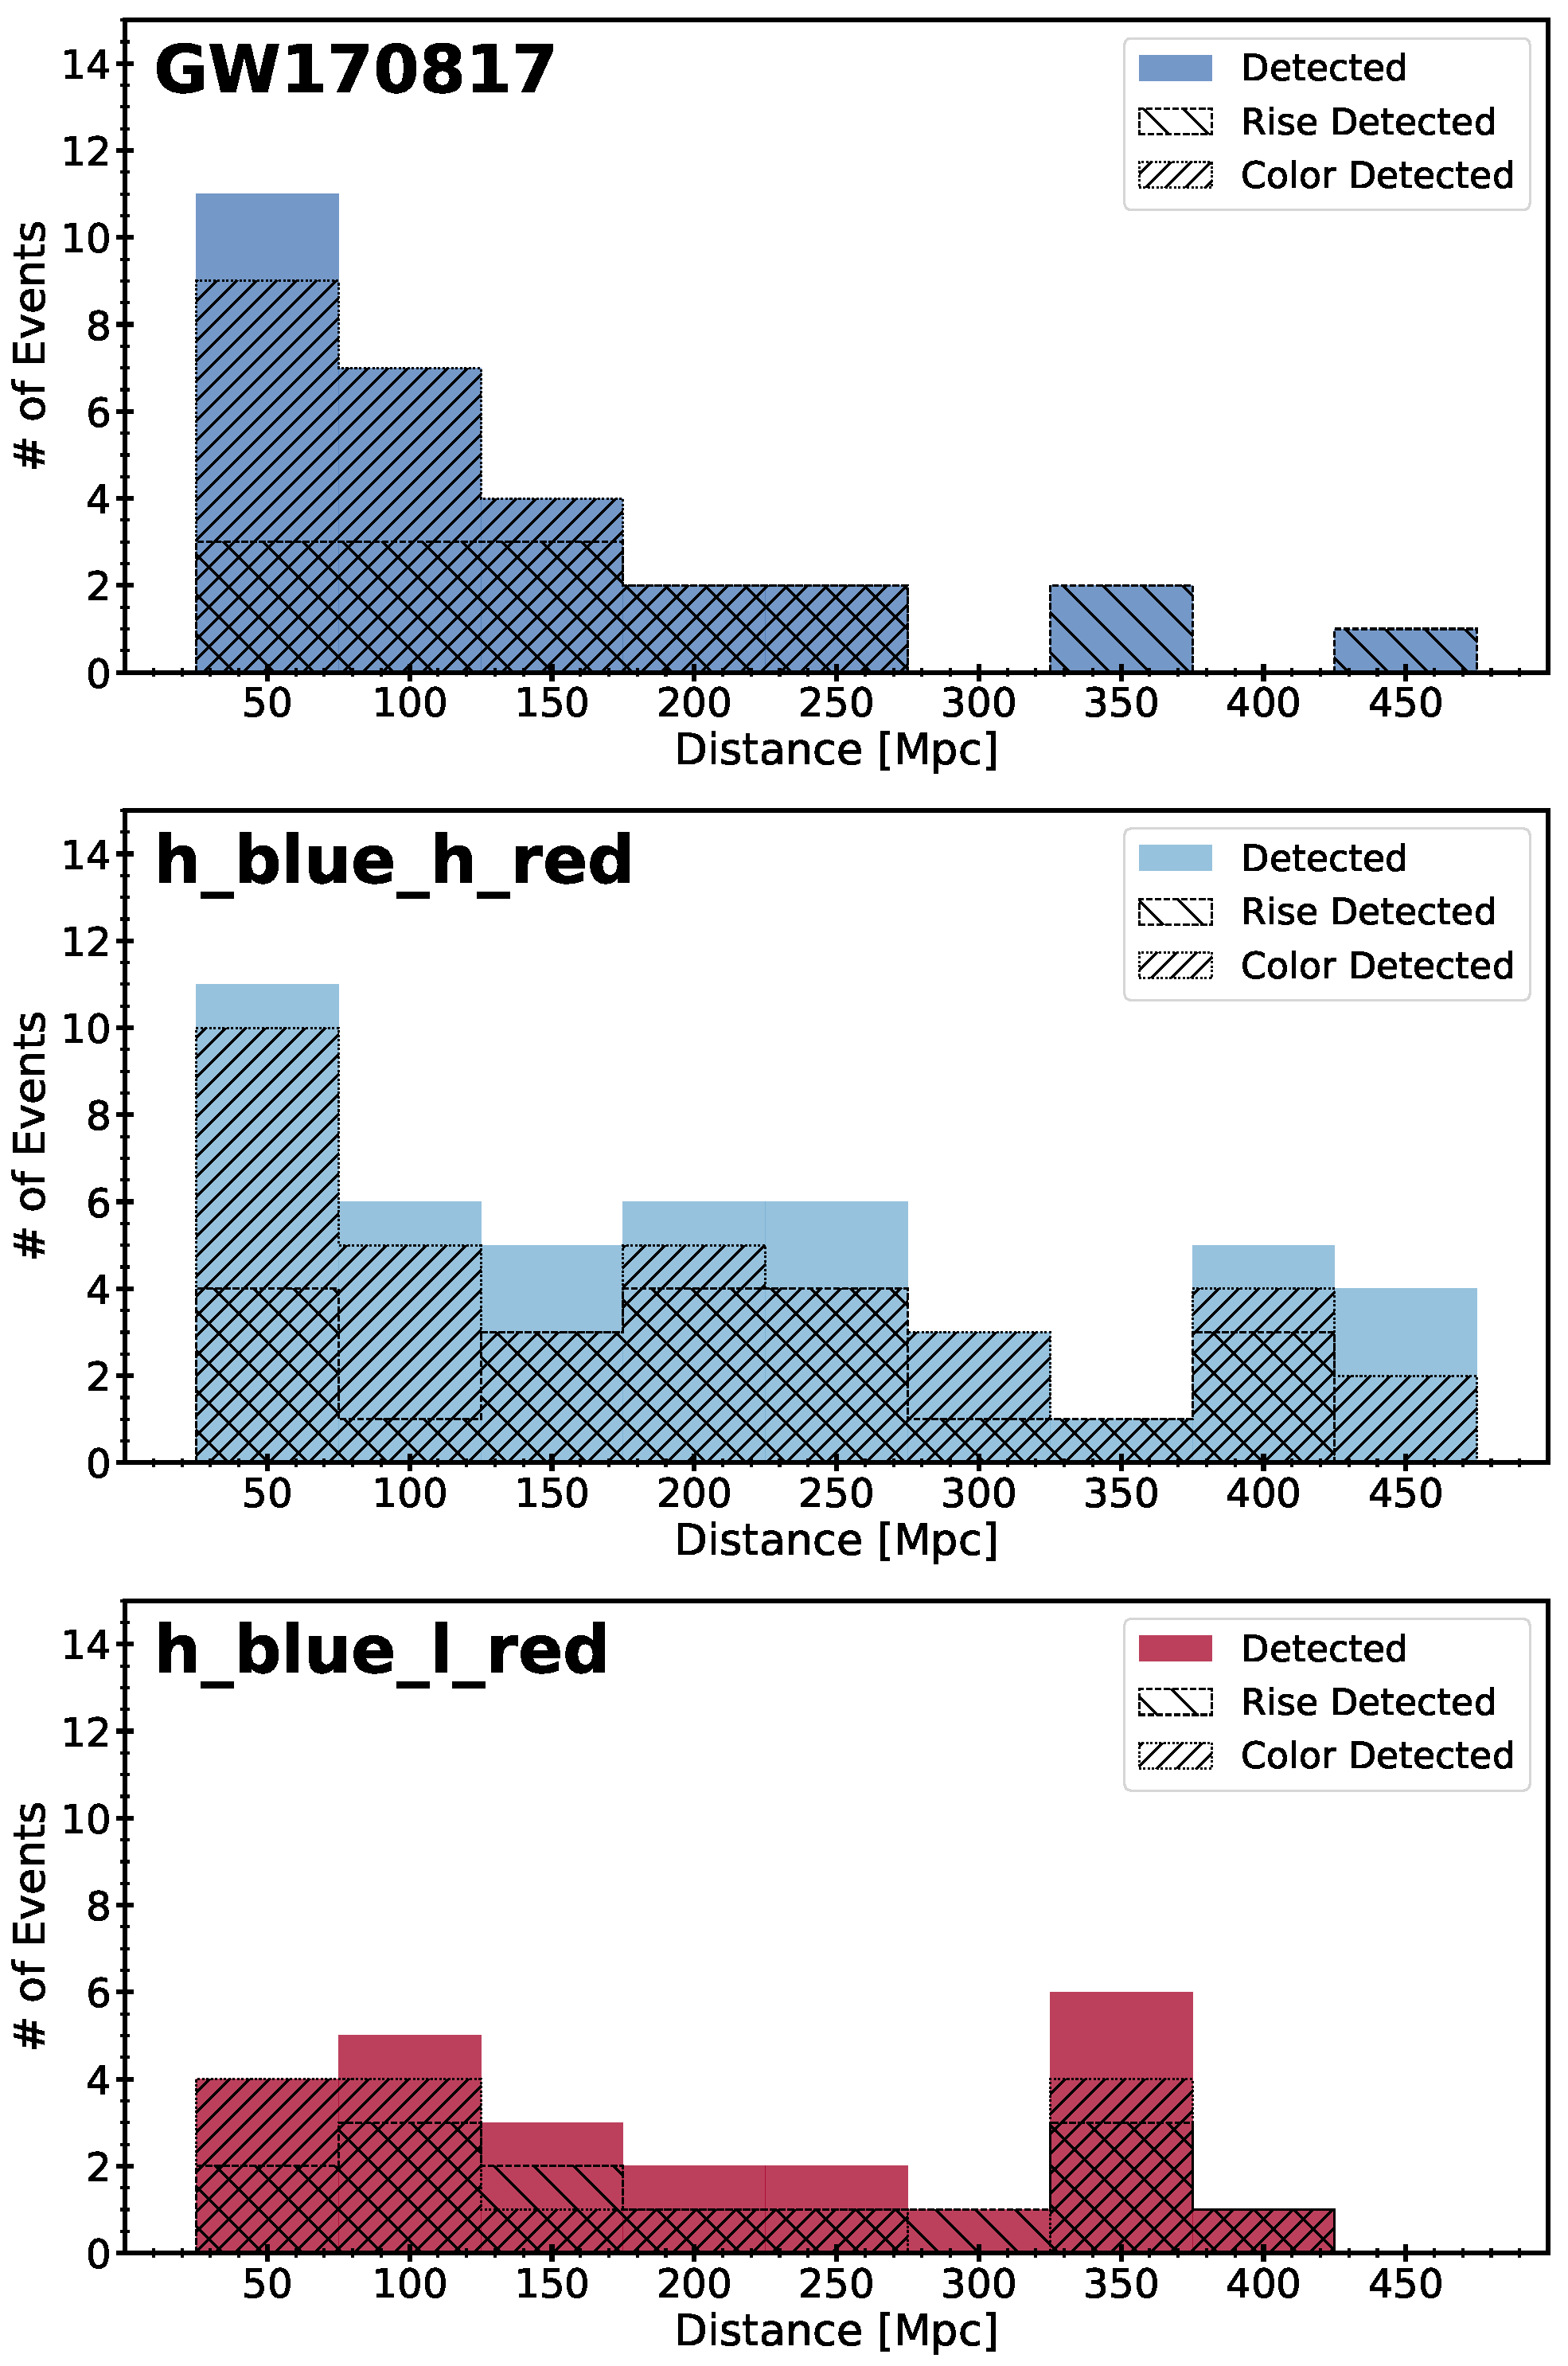
\includegraphics[width=0.75\textwidth]{./figs/chapter6/f1.pdf}}
%\caption{\singlespace Histograms showing the number of detections as a function of model and distance, for those models that are detected. We note that as a result of the cadence of the LSST main survey we are not always able to obtain crucial information about the rise and color.}
%\label{fig:ch6_eff_hist}
%\end{center}
%\end{figure}

\clearpage
Looking at \Cref{fig:ch6_eff_hist} and \cref{tab:ch6_eff}, we first note that only the three brightest models (GW170817, {\tt h\_blue\_h\_red}, and {\tt h\_blue\_l\_red}) are detected. The model {\tt l\_blue\_h\_red}, is not detected despite having the same {\it total} ejecta mass as the model {\tt h\_blue\_l\_red}. This is because all the mass in the {\tt l\_blue\_h\_red} is contained in the high-opacity ``red" component and is therefore less luminous. The model {\tt l\_red\_l\_blue} is simply too faint to detect due to it's extremely low total ejecta mass.  Inspecting \Cref{fig:ch6_eff_hist} for trends that depend on distance, we note that the models for GW170817 and {\tt h\_blue\_h\_red} are preferentially detected at small distances ($D_L \lesssim 100$~Mpc). There is a similar trend for detecting brightening in these models, however there is no strong dependence on distance and the availability of color information. The model {\tt h\_blue\_l\_red} shows no strong dependence on distance for any criteria.

We also investigate the timing of our detections by defining two crucial times. The value $t_{\rm first}$ is the time, in days, from explosion to the first observation with S/N $> 5$, while $t_{\rm last}$ is the time from explosion to the last observation with S/N $> 5$. The number of events as a function of these two values are shown in \Cref{fig:ch6_t_hist}. Looking at the distribution with respect to $t_{\rm first}$, we find a slight preference for detections at early times particularly for the model of GW170817.  We also find that the latest value of $t_{\rm first}$ is \apx$5-6$~days for all three models. Looking at the distribution with respect to $t_{\rm last}$, we first find that in general the last observation is obtained within a week of explosion. The only exception is GW170817, where a handful of events are detected out to two weeks post explosion. We also note that 4 events have a value of $t_{\rm last}$ of $\lesssim 1$~day. These events appeared in high cadence regions of the survey, resulting in 4-5 observations being obtained in a single night. The sky positions of these events do not correspond to the LSST deep drilling fields, but rather a spurious increases in observing cadence.

%\begin{figure}[!t]
%\begin{center}
%\hspace*{-0.1in}
%\scalebox{1.}
%{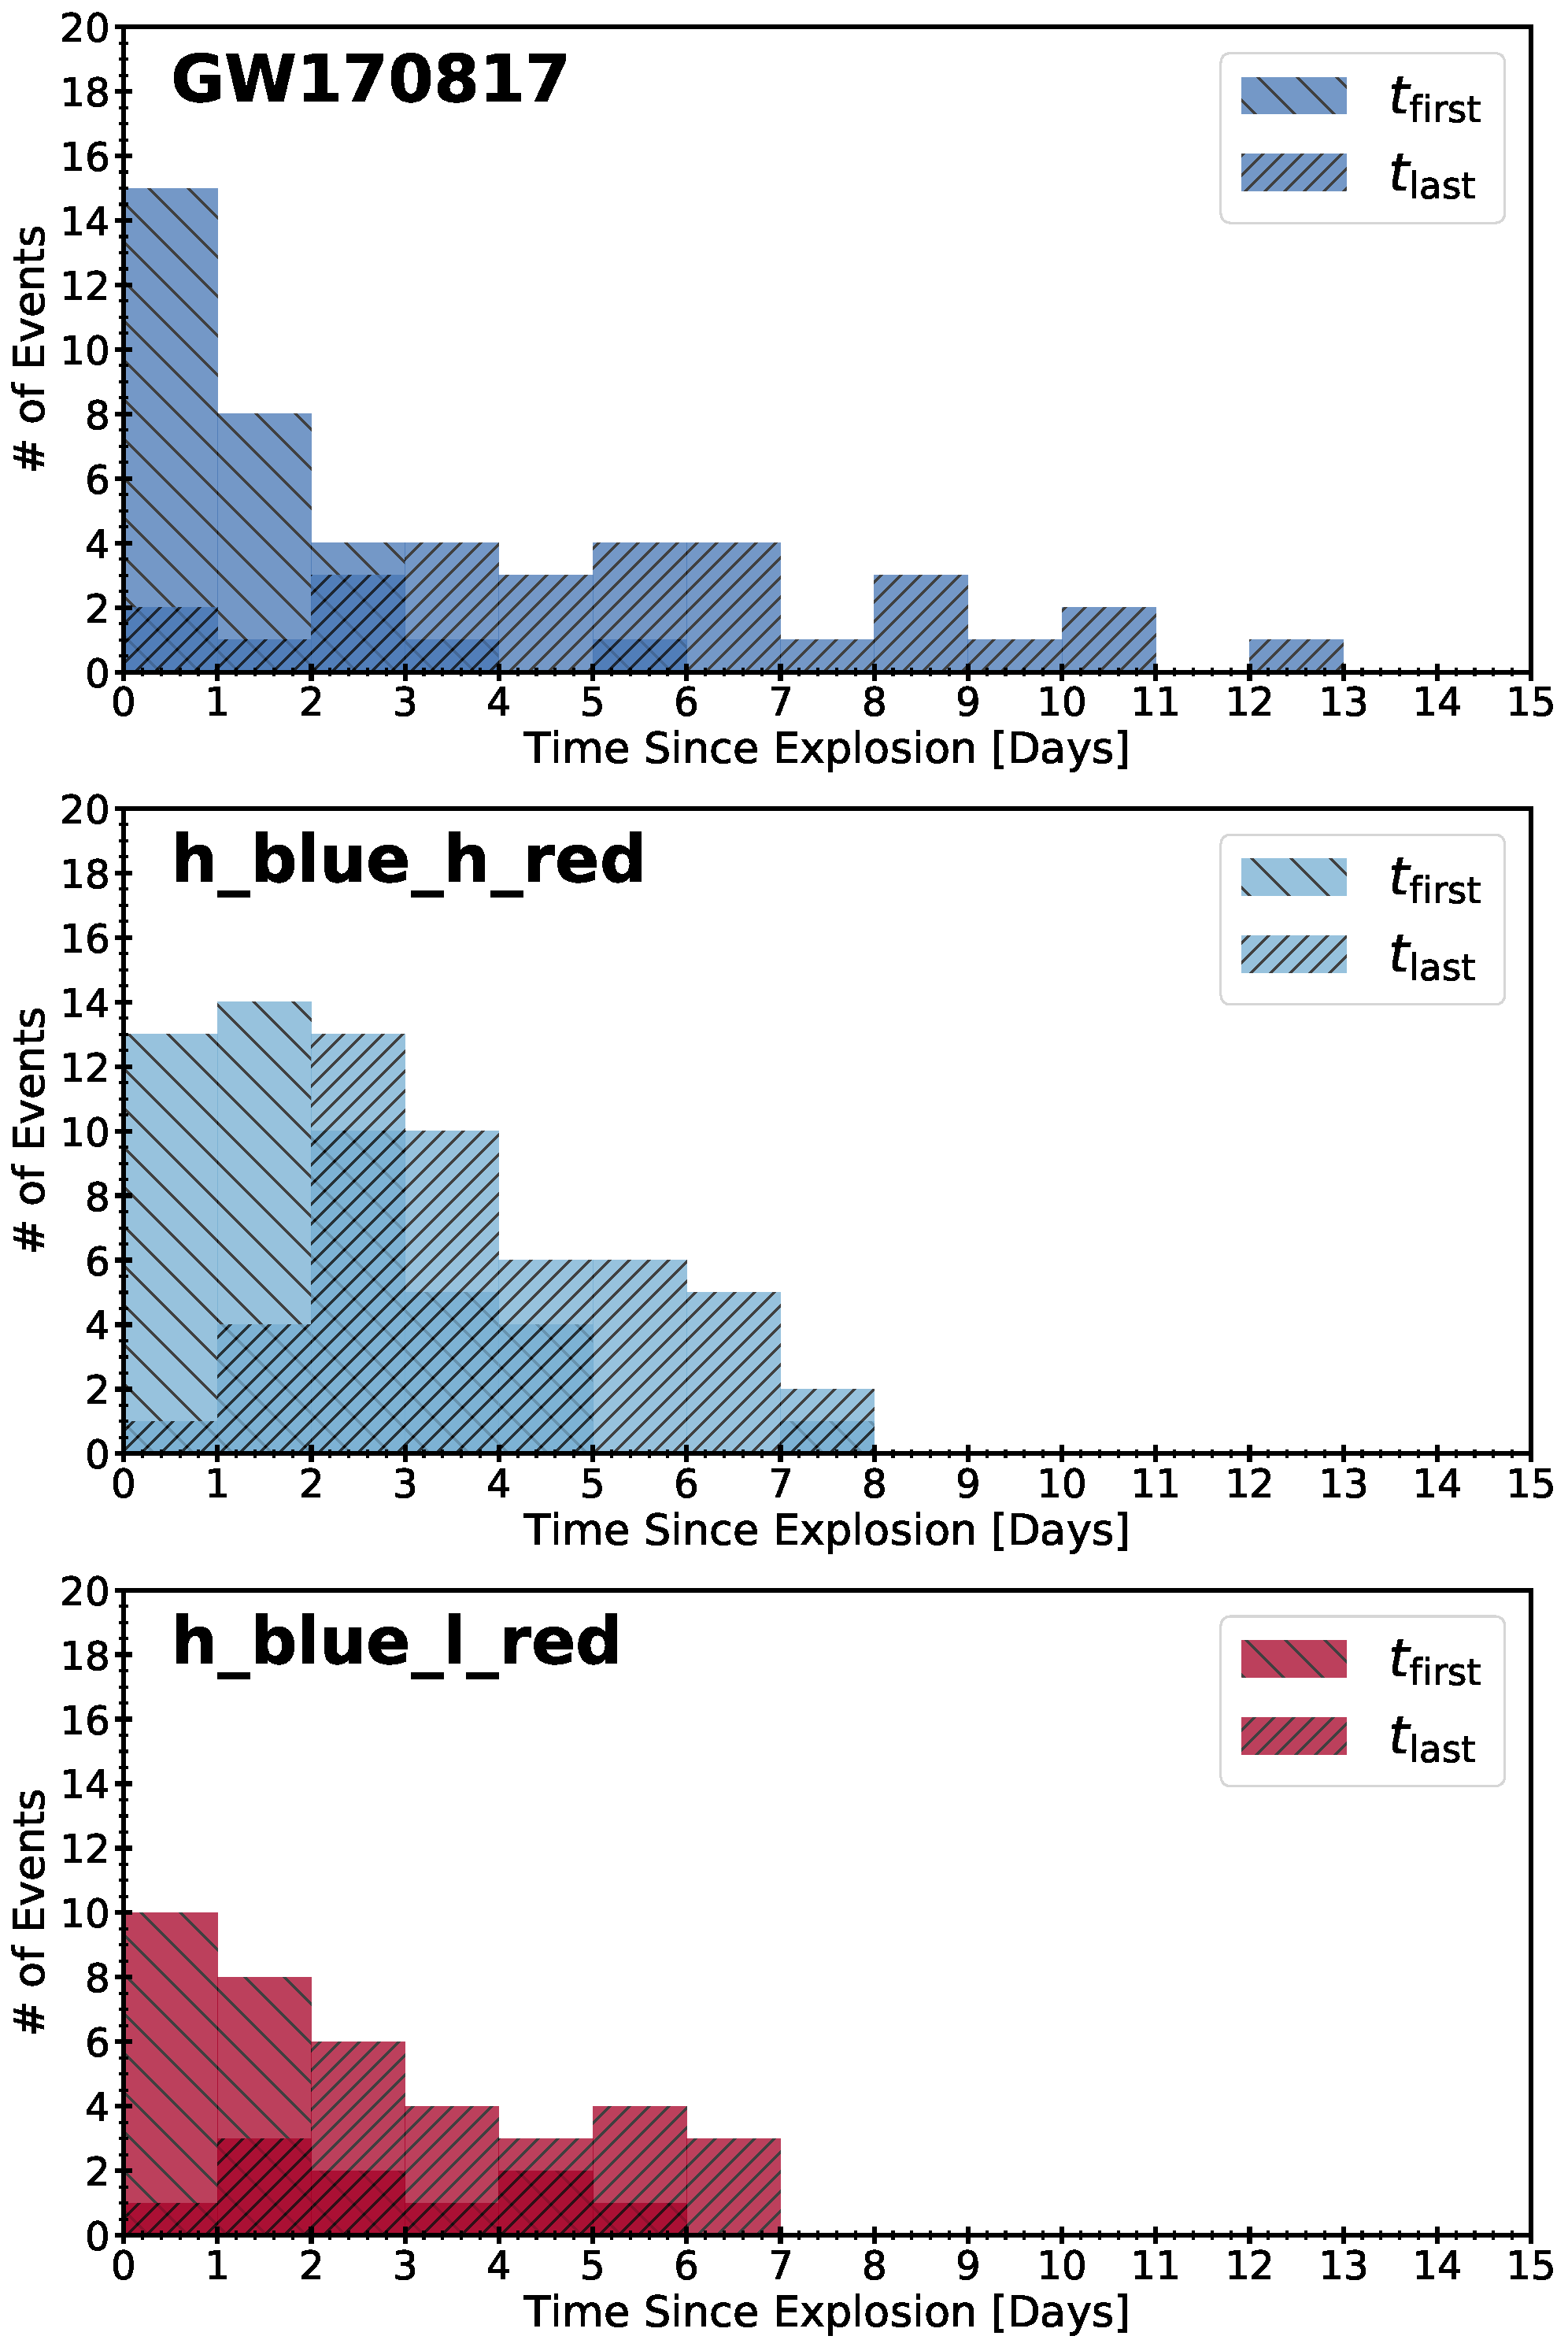
\includegraphics[width=0.725\textwidth]{./figs/chapter6/f2.pdf}}
%\caption{\singlespace Histogram of events as a function of time to first or last detection. As with \Cref{fig:ch6_eff_hist}, we only plot those models that are detected. The LSST main cadence is only able to track a limited number of events out to longer times than \apx~a few days. This combined with the poor rise and color constraints shown in \Cref{fig:ch6_eff_hist} means that kilonovae detected in the LSST main survey will be difficult to detect and characterize.}
%\label{fig:ch6_t_hist}
%\end{center}
%\end{figure}

Lastly, we are concerned with the overall efficiency of our search. This is shown as a function of distance and model in \Cref{fig:ch6_dist_eff}. As expected, the survey achieves the highest efficiency for nearby sources $(D_L \apx50$~Mpc). If we only consider injected sources that were observed by LSST, we compute a model averaged efficiency of \apx26\%. If we exclude models that are never detected, this efficiency rises to \apx48\%. This efficiency drops sharply to \apx15\% at a distance of $D_L \apx250$~Mpc, beyond which the efficiency shows no strong dependence on distance. The efficiency averaged over the entire volume considered is \apx11\% for all models, and \apx17\% when considering only detected models.

%\begin{figure}[!t]
%\begin{center}
%\hspace*{-0.1in}
%\scalebox{1.}
%{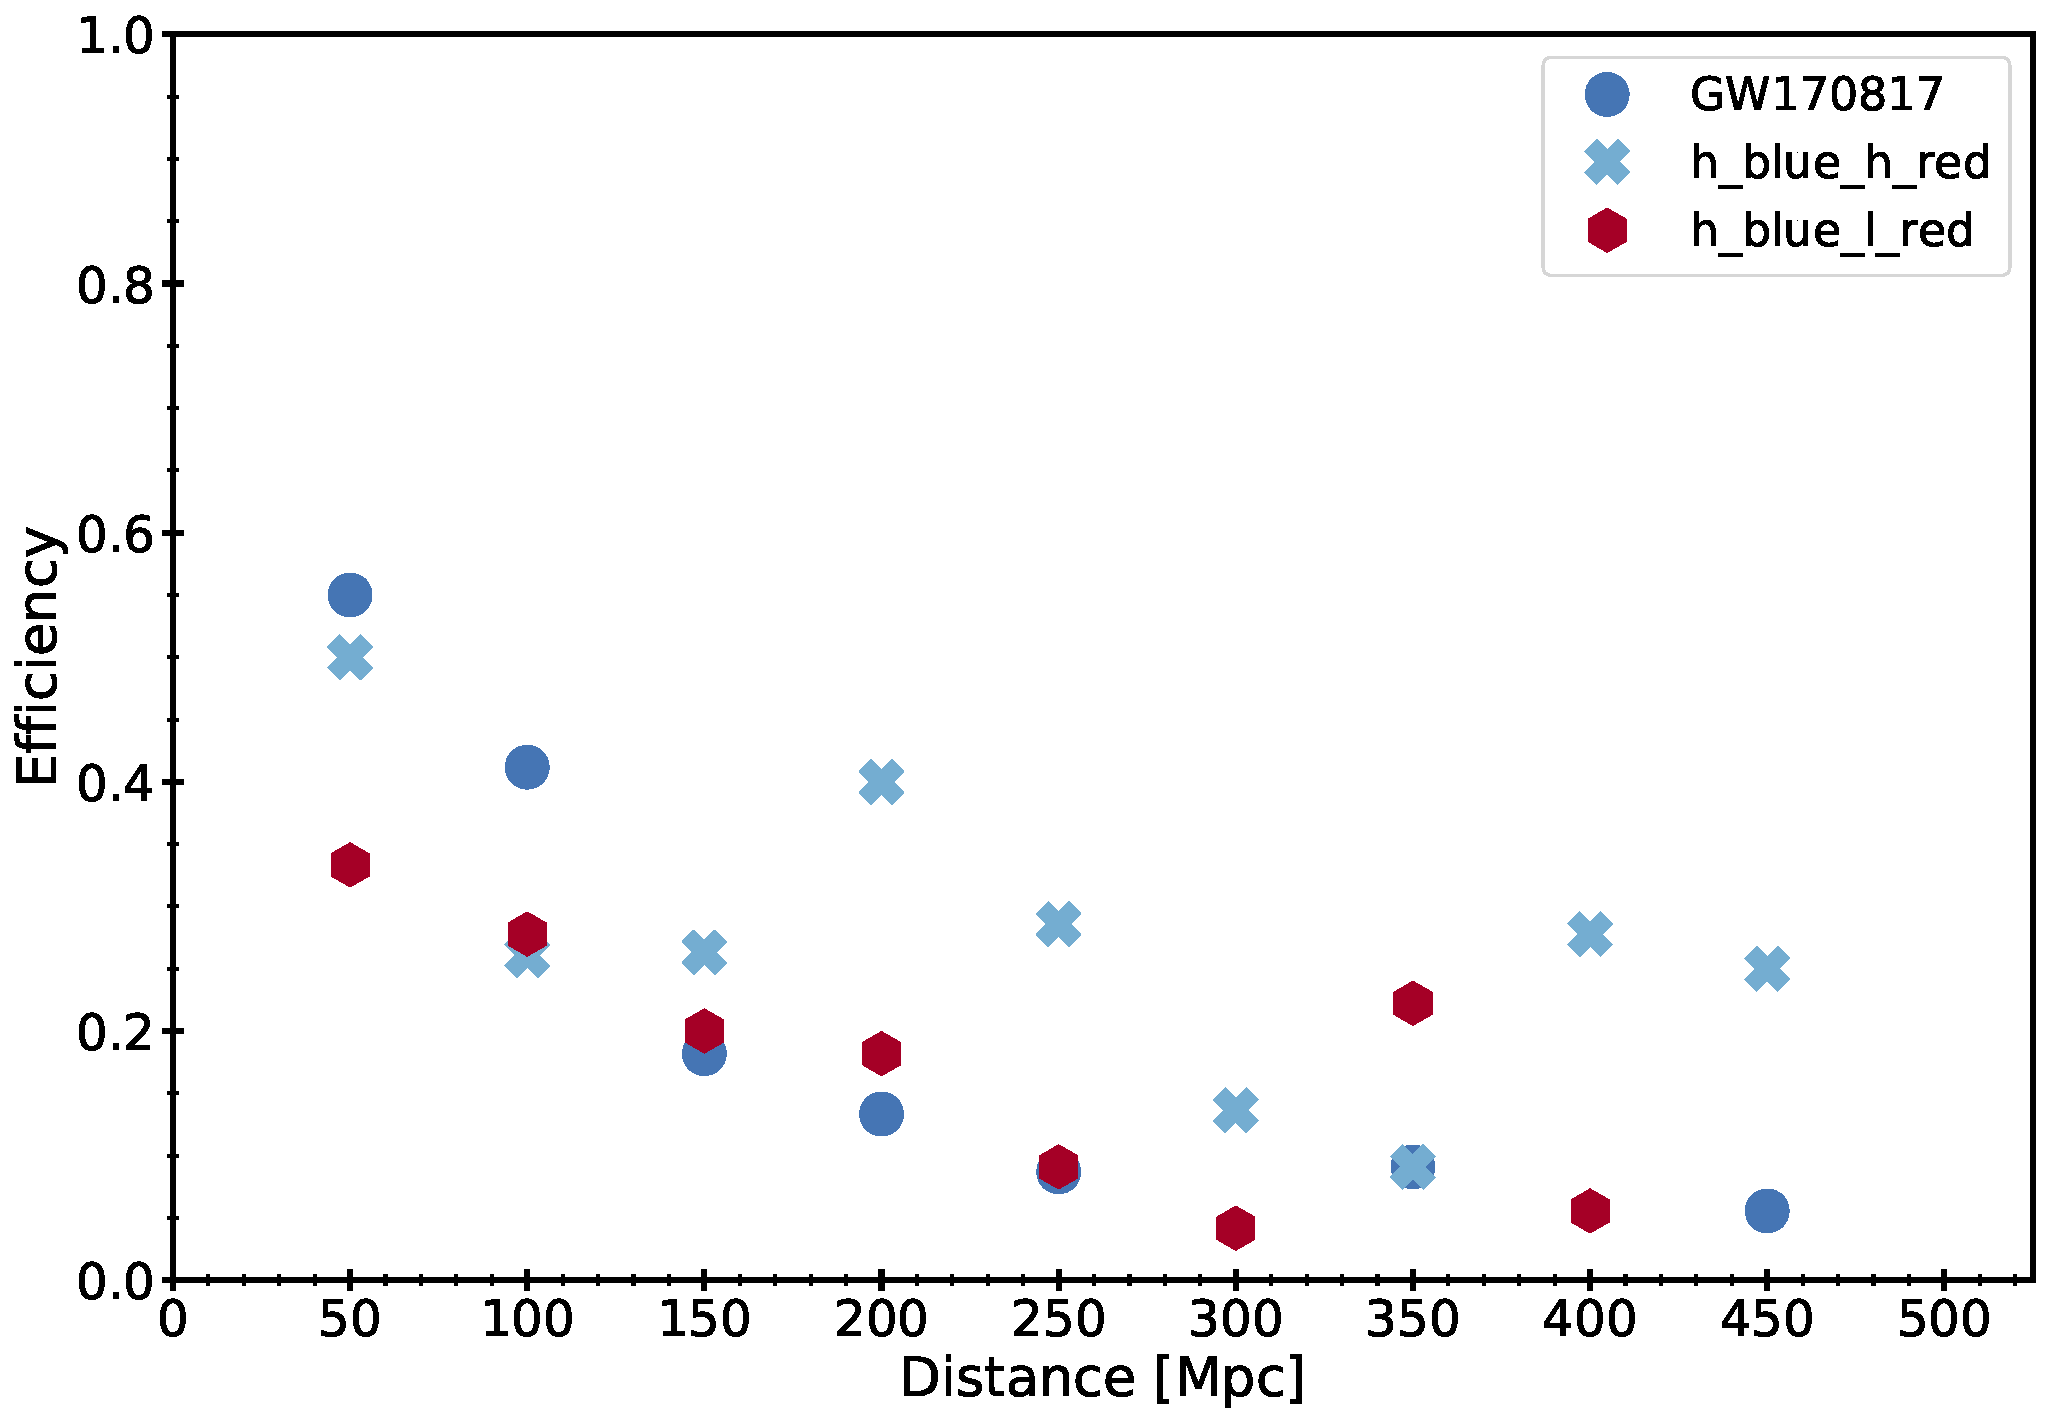
\includegraphics[width=0.9\textwidth]{./figs/chapter6/f3.pdf}}
%\caption{\singlespace Detection efficiency as a function of distance for each of the detected models. As expected, the efficiency is high (\apx45\%) for nearby sources ($D_L \apx50$~Mpc), but rapidly tapers off to \apx15\% at the edge of the LIGO BNS detection range $(D_L \gtrsim 400$~Mpc).}
%\label{fig:ch6_dist_eff}
%\end{center}
%\end{figure}

We now wish to compute the total number of kilonovae we expect to detect in our search volume over the course of the LSST main survey. We compute this number using the following expression:
\begin{equation}
N_{\rm tot} = 4 \pi \mathcal{R} \int \epsilon (z) \frac{dV}{dz} dz,
\end{equation}

\noindent where $\mathcal{R}$ is the expected rate of kilonovae, $\epsilon (z)$ is the efficiency as a function of distance, and $dV/dz$ is the differential comoving volume \citep[see e.g.,][]{Hogg1999}. The factor of $4\pi$ accounts for the fact that $dV/dz$ has units of Mpc$^{3}$ sr$^{-1}$ and indicates we are considering the number of kilonovae across the entire sky. We assume the rate of kilonovae is the rate of BNS mergers derived by LIGO during the second observing run \citep[$\mathcal{R} \apx1500$~Mpc$^{-3}$~yr$^{-1}$,][]{LIGOGW170817}. Here we compute the efficiency, $\epsilon (z)$, using the total number of kilonovae injected in each distance bin. We find a total expected number of $N_{\rm tot} \approx 8.8$ kilonovae per year across the entire ten year survey. This number is comparable to that found by \citet{Scolnic+18}. If we compute $\epsilon (z)$ by only considering sources for which there is both rise and color information, then we find $N_{\rm tot} \approx 3.6$ kilonovae per year.

The key point emerging from this study is that despite the large \'{e}tendue of the LSST survey, it will be relatively inefficient at finding kilonova compared to other types of transient events. More importantly, the small number of kilonovae that will have sufficient light curve data for more detailed studies suggests that the science returns for each event will be low. This low efficiency also suggests that the likelihood of a serendipitous joint detection between LIGO and LSST is vanishingly small. Even in the fortuitous situation of a joint detection, if it takes several days to detect and identify the kilonovae, this will severely limit our ability to perform multi-wavelength imaging and spectroscopy. These comprehensive multi-wavelength follow-up programs were found to be crucial for maximizing the science returns from GW170817.

\subsection{Results from SNANA}
\label{sec:ch6_snana_results}
We analyze the sample of light curves from our SNANA simulations using the same criteria outlined in \cref{sec:ch6_opsim_results}, with one key change: we now require that brightening be detected between observations taken in the same filter. This is necessary as our broadband imaging on a single night will sample the kilonova SED well enough that erroneous "brightening" will be detected between filters. We apply these criteria to our sample of light curves finding that as with the OpSim simulations, we are only able to detect the three brightest kilonovae models. This is expected given that our ToO observations still use the same exposure time as OpSim (30~s), so even with an improved cadence and broadband coverage the models {\tt l\_blue\_h\_red} and {\tt l\_blue\_h\_red} are simply not bright enough to detect without deeper exposures.

The detection efficiency as a function of distance is shown in \Cref{fig:ch6_snana_dist_eff}. We first note that the efficiency is flat as a function of distance with a model-averaged efficiency of \apx20\%. It is important to note however, that this number is computed using all injected sources. If we consider only those models for which there is at least one detection, then the efficiency is 100\% at all distances. Furthermore, as a result of the nightly broadband imaging we are able to obtain color information for all detected kilonovae. However, we find that our ability to detect brightening in the light curve is poor, with an average efficiency of \apx10\%. This efficiency shows no strong dependence on distance, suggesting that other factors such as the promptness of observations are important.

%\begin{figure}[!t]
%\begin{center}
%\hspace*{-0.1in}
%\scalebox{1.}
%{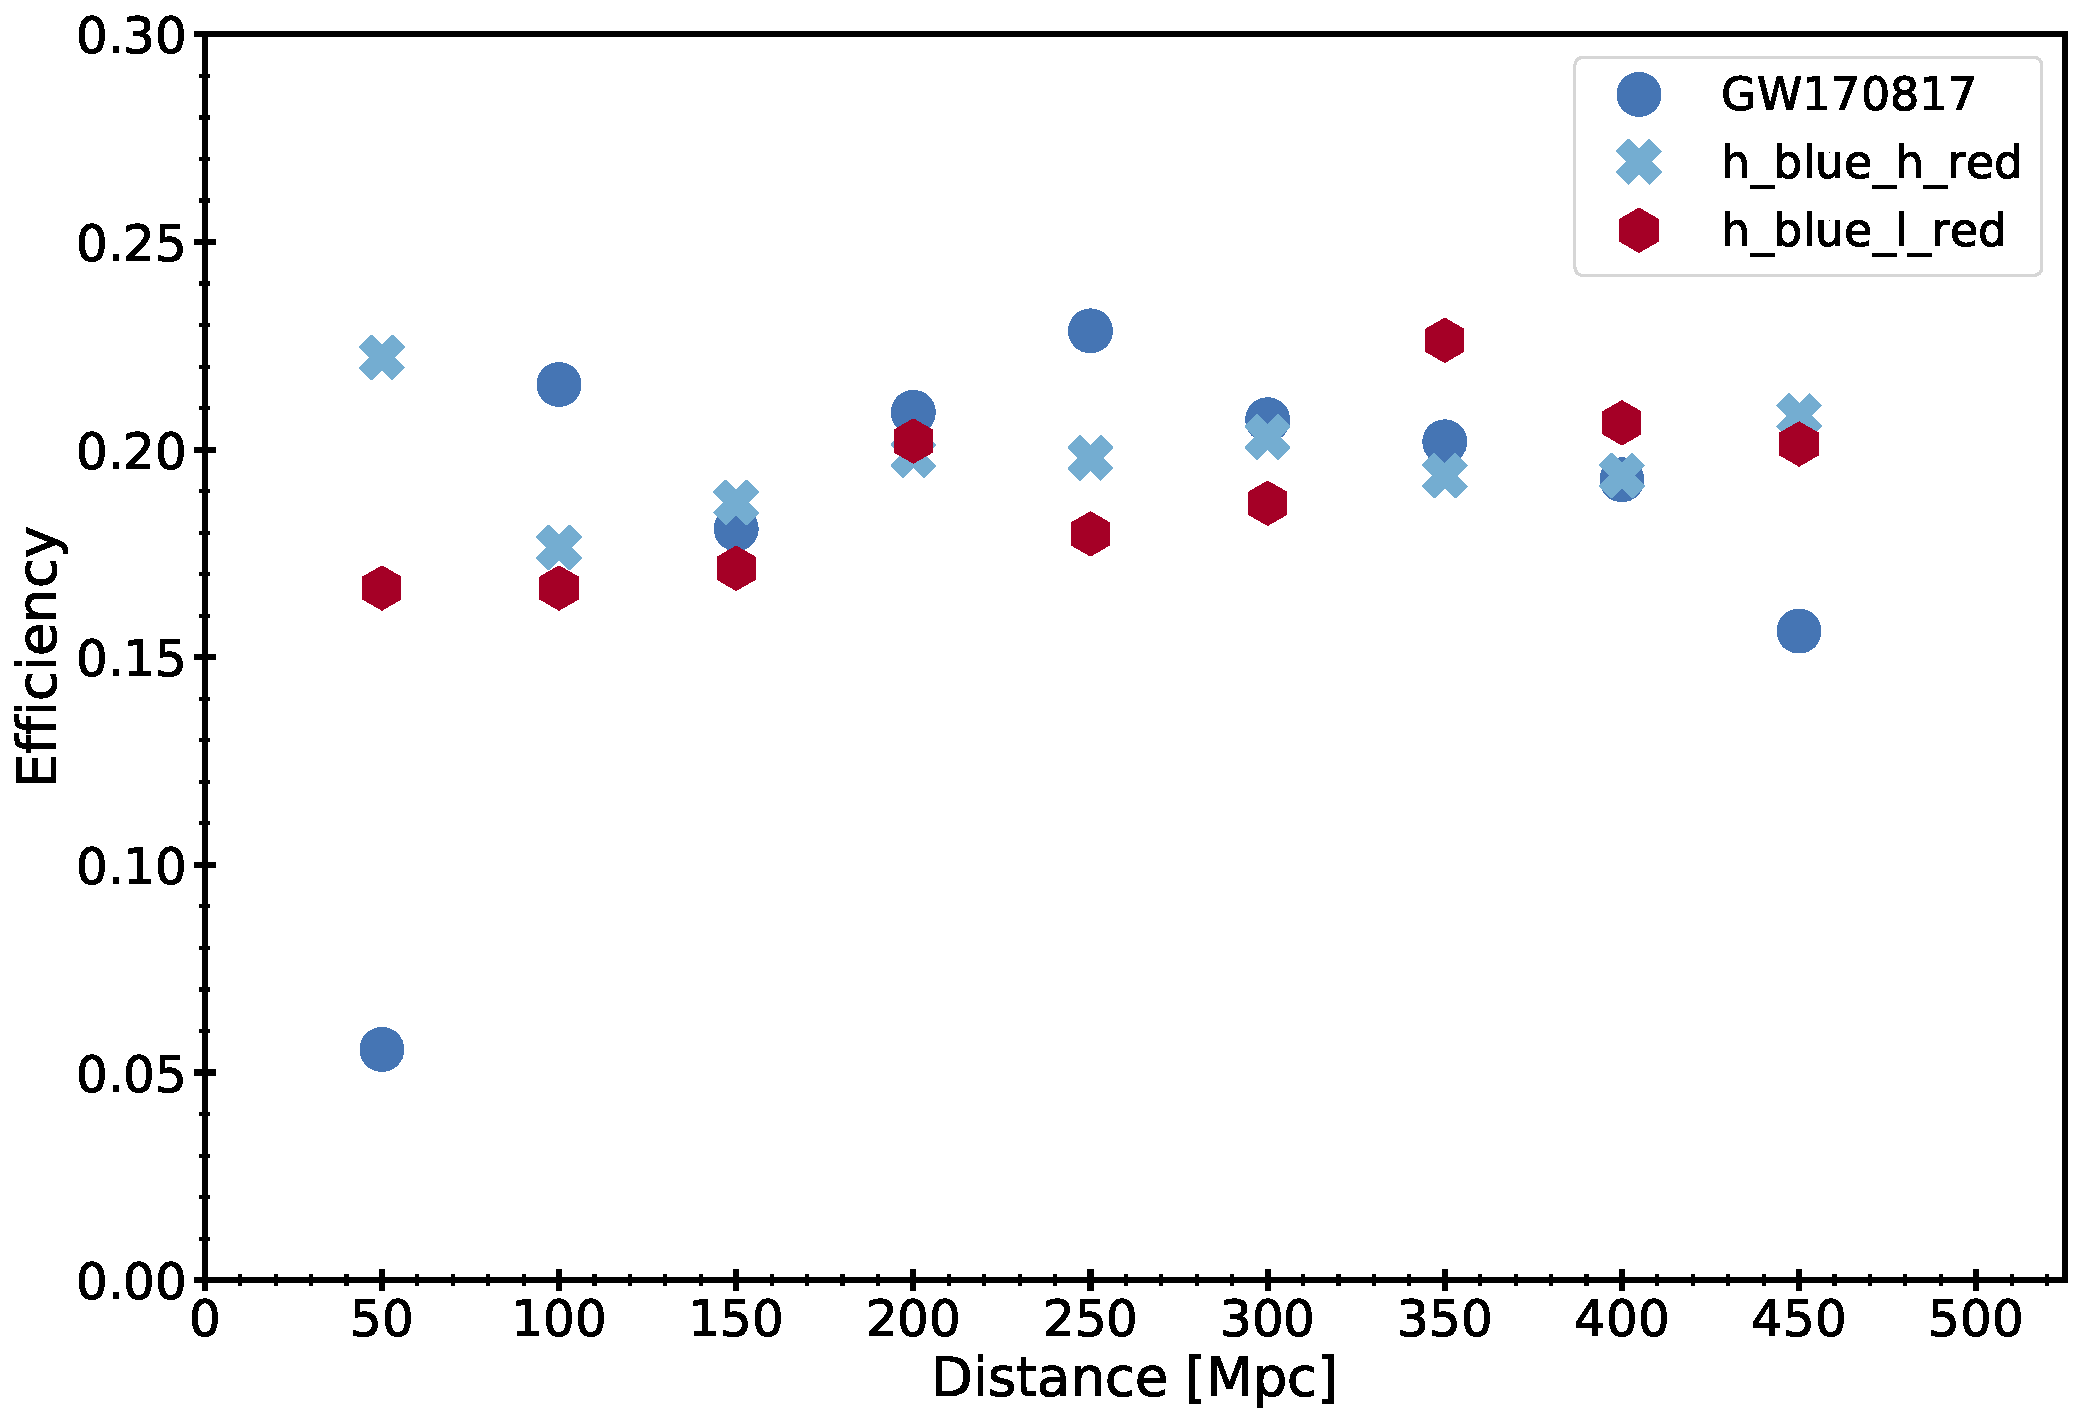
\includegraphics[width=0.9\textwidth]{./figs/chapter6/f5.pdf}}
%\caption{\singlespace Efficiency of our ToO searches as a function of distance. The numbers plotted here are relative to the total number of injected sources (i.e., including models not detected). The {\it per model} detection efficiency is 100\% for the bright KN models plotted. The efficiency curve is flat as a function of distance indicating that ToO efforts with LSST can be effective out to the maximal LIGO BNS detection distance.}
%\label{fig:ch6_snana_dist_eff}
%\end{center}
%\end{figure}

We investigate this by computing our efficiency as a function of time, in hours, between the time of explosion and the time of our first observation. We first note that the overall detection efficiency is not affected by the start time of our observations. We again achieve a model-averaged efficiency of \apx20\% when considering all injected sources, and an efficiency of 100\% when only considering the models for which we have detections. However, we do find that our ability to detect brightening in the light curve is strongly impacting by the start time of observations. This can be seen in \Cref{fig:ch6_snana_t_eff} which shows the fraction of detected sources that also exhibit brightening in at least one filter. For observations that start promptly (+3~hours), then brightening can be detected in 60\% of sources. This however, plummets quickly to \apx5\% at +9 hours, and 0\% at later times. This highlights the fact that rapid response must be a priority for any triggered ToO program to be successful.

%\begin{figure}[!t]
%\begin{center}
%\hspace*{-0.1in}
%\scalebox{1.}
%{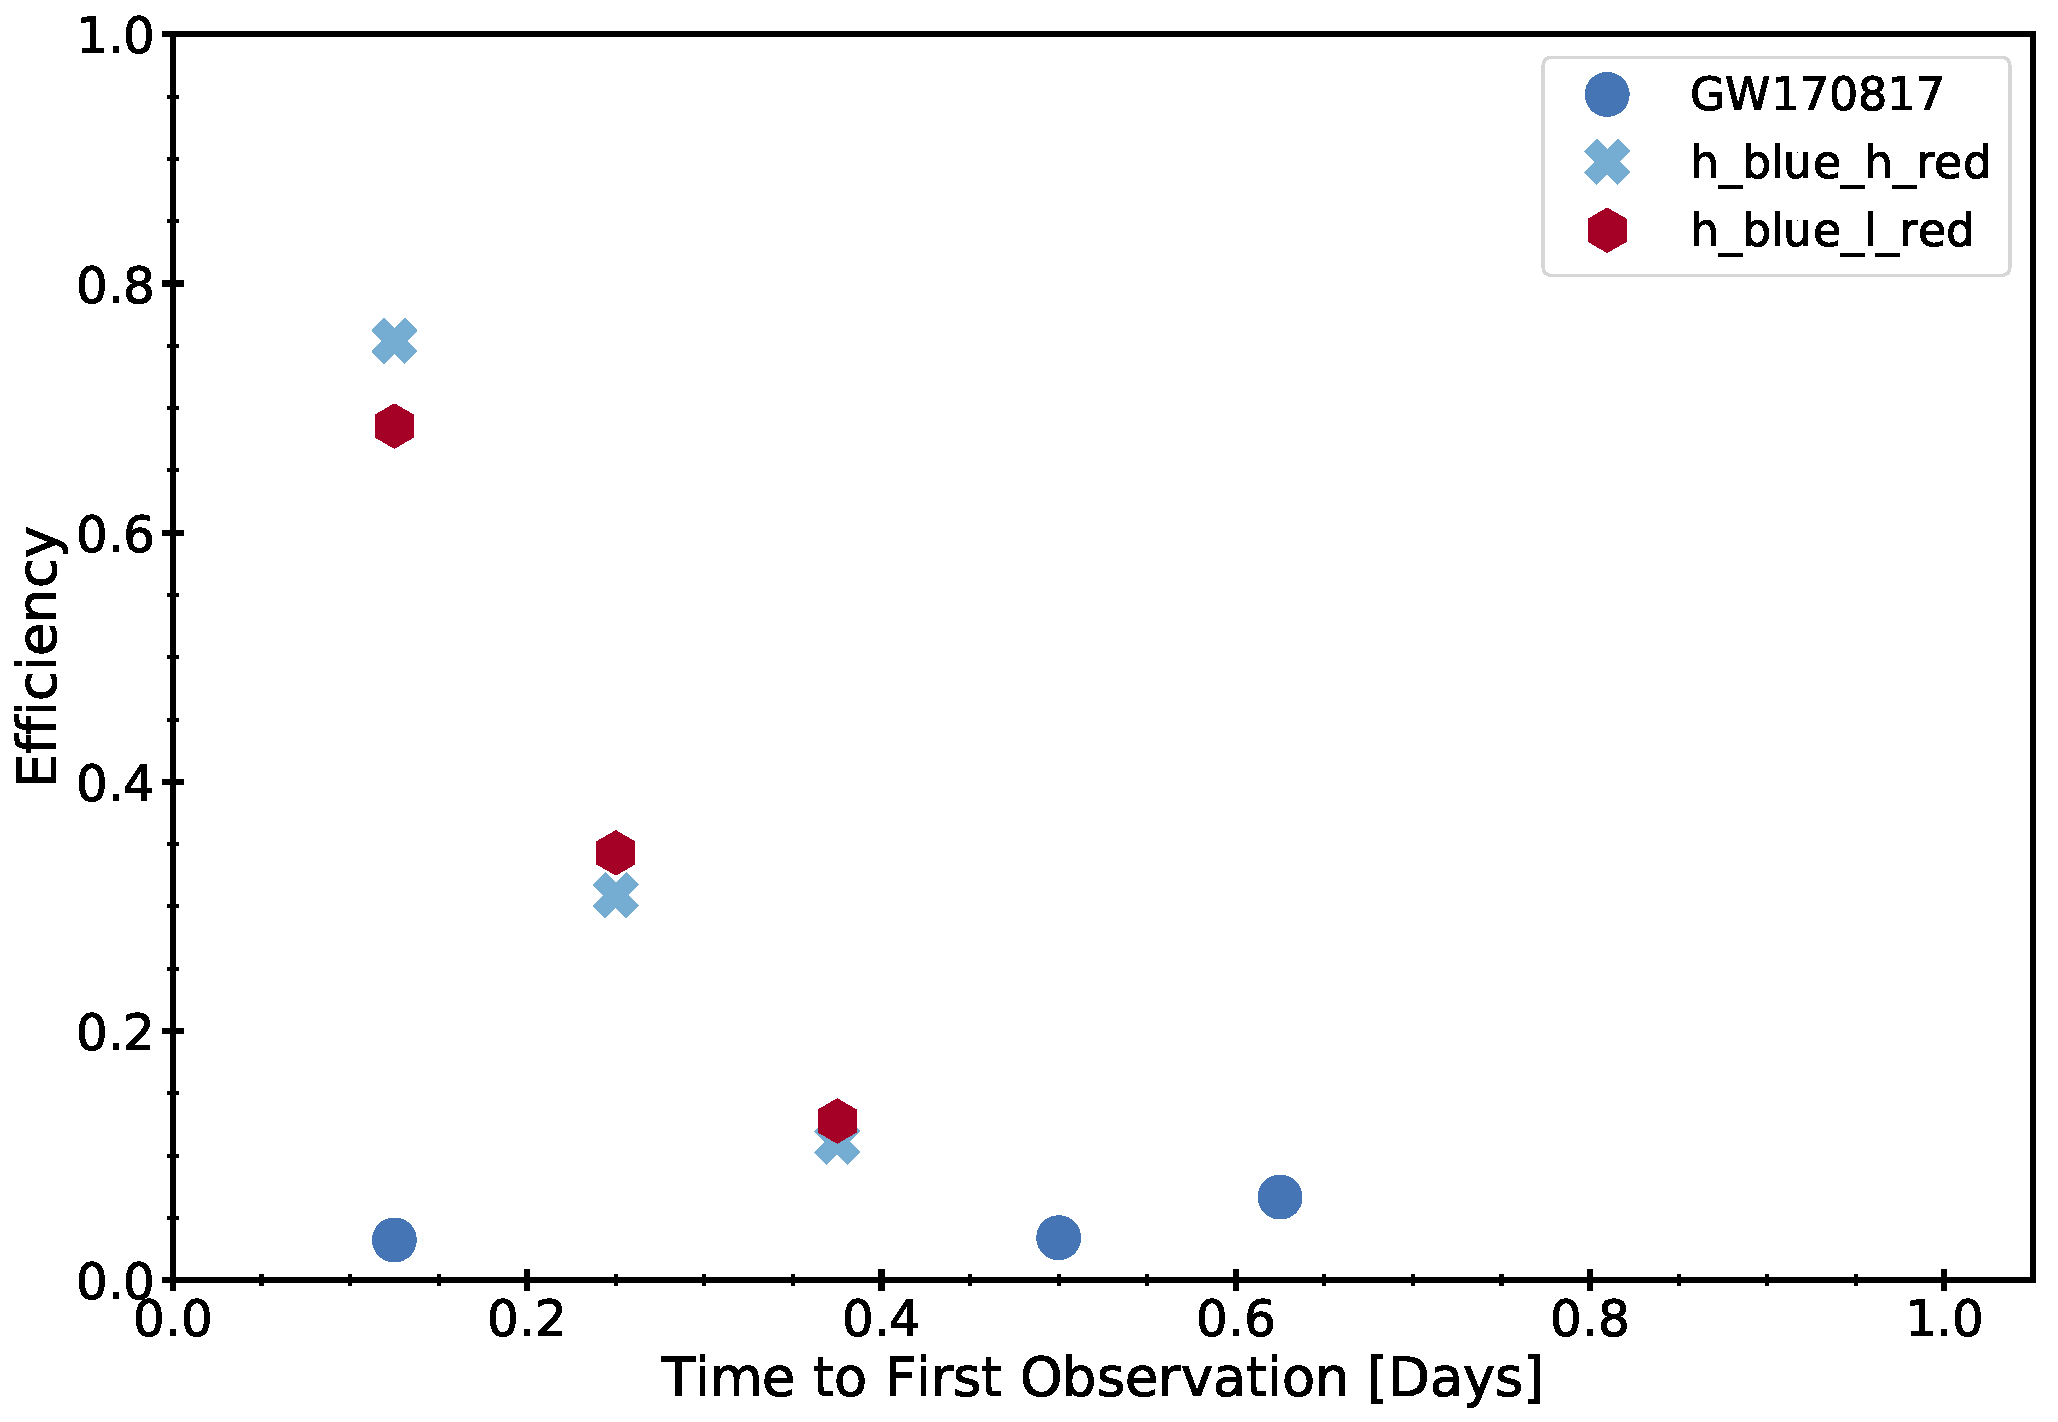
\includegraphics[width=0.9\textwidth]{./figs/chapter6/f6.pdf}}
%\caption{\singlespace Efficiency of our ToO searches to detect brightening in the kilonova light curve in at least one filter as a function of starting time. The efficiency here is computed relative to the number of detected sources in a given time bin $(\Delta_t \apx3$~hrs). There is a sharp drop off in efficiency after just a few hours. This efficiency drops to 0 under all observing scenarios when just a single epoch is obtained on the first night.}
%\label{fig:ch6_snana_t_eff}
%\end{center}
%\end{figure}

Lastly, we consider the effect of altering our ToO cadence and telescope time investment in our computed efficiencies. First, we investigate the effect of removing the second epoch from the first night of observations. This has no impact on our general ability to detect kilonovae, resulting in identical efficiency calculations. There is however, a strong impact on our ability to detect the kilonova rise. When observations are conducted without the second epoch on the first night, the efficiency for detecting brightening drops to 0\% for all models, at all distances and all start times. The second rapid epoch is therefore crucial for characterizing the early light curve behavior. Second, we investigate the effect of truncating the total time spent observing to 3 or 5 days per event. This is accomplished by taking the simulated light curves, removing epochs after the truncation time, and recomputing all of our criteria. We find that truncating our light curves does not alter our efficiency calculations. This suggests that just 20 minutes a night for 3 nights (e.g., one hour total telescope time) is sufficient to detect the brightest kilonovae out to the maximal LIGO BNS detection range. Candidates identified in this manner could be passed off to other facilities for targeted follow-up (e.g., deep imaging and spectroscopy) allowing LSST to quickly return to normal science operations.

\section{Discussion and Conclusion}
\label{sec:ch6_conc}
We have presented detailed simulated observations of kilonovae using LSST in two distinct contexts. First, we investigated the ability of LSST to both detect and characterize kilonovae over the course of the primary ten year survey. Second, we investigate the effectiveness of a triggered target-of-opportunity campaign conducted in response to a gravitational wave event trigger from the Advanced LIGO/Virgo interferometers. A key point that emerges from both studies is that it may be difficult to detect kilonova across the entire range of possible ejecta parameters. Models that have ejecta masses similar to or greater than those associated with GW170817 can be detected by LSST. However, models with less ejecta mass quickly become too faint to observe effectively. We further find:

\begin{enumerate}
\item We find that the LSST main survey has an average efficiency for kilonova detection of \apx3\%. This efficiency is strongly a function of distance, peaking for nearby sources $(D_L \lesssim 100$~Mpc). Using this efficiency, we find that LSST will detect \apx8.8 kilonovae per year in the main survey over ten years. However, if we consider our efficiency for sources with enough light curve information to perform detailed studies, this number drops to \apx3.6 kilonovae per year.
\item We find that triggered ToO observations with LSST can be highly effective at detecting and characterizing kilonovae compared to the main survey cadence. ToO campaigns involving just an hour of telescope time are able to achieve a model-averaged efficiency of \apx45\%. This efficiency is 100\% for the brightest kilonova models. A key concern is prompt scheduling of observations in response to a trigger, as crucial early time behavior is difficult to capture for observations starting later than \apx3-6 hours post-explosion.
\end{enumerate}

Most importantly, we have shown that the cadence of the LSST main survey is poorly matched to kilonovae timescales, leading to just a handful of detections per year. However, targeted ToO campaigns with a modest investment in telescope time (\apx1~hour) can detect the brightest kilonovae models across the entire Advanced LIGO/Virgin volume. An increase in this time investment by a factor of 2 to account for deeper exposures will allow LSST to probe the faintest kilonovae models at a level that is simply not possible with other ground-based survey instruments. Therefore, it is clear that LSST can and should play a vital and important role in the future of joint GW-EM astronomy. 
%NO BIB INFO